\documentclass[conference]{IEEEtran}
\IEEEoverridecommandlockouts

\usepackage{cite}
\usepackage{amsmath,amssymb,amsfonts}
\usepackage{graphicx}
\usepackage{booktabs}
\usepackage{multirow}
\usepackage{algorithm}
\usepackage[noend]{algpseudocode}
\usepackage{tikz}
\usetikzlibrary{positioning,arrows.meta,fit,calc}
\usepackage{xcolor}
\usepackage{url}

\newtheorem{proposition}{Proposition}
\newcommand{\amdie}{\textsc{amdie}}

\begin{document}

\title{BizTwin AI: An Adaptive Multi-Agent Decision Intelligence Engine for Small and Medium Business Operations}

\author{
\IEEEauthorblockN{Ms. D. Brindha}
\IEEEauthorblockA{\textit{Assistant Professor}\\
\textit{Dept. of Artificial Intelligence and Data Science}\\
\textit{Dr. N.G.P Institute of Technology}\\
Coimbatore, India\\
brindha.d@drngpit.ac.in}
\and
\IEEEauthorblockN{Pranesh S}
\IEEEauthorblockA{\textit{UG Student}\\
\textit{Dept. of Artificial Intelligence and Data Science}\\
\textit{Dr. N.G.P Institute of Technology}\\
Coimbatore, India\\
23ad080@drngpit.ac.in}
\and
\IEEEauthorblockN{Sanjai M}
\IEEEauthorblockA{\textit{UG Student}\\
\textit{Dept. of Artificial Intelligence and Data Science}\\
\textit{Dr. N.G.P Institute of Technology}\\
Coimbatore, India\\
23ad094@drngpit.ac.in}
\and
\IEEEauthorblockN{Shri Subeesesh V K}
\IEEEauthorblockA{\textit{UG Student}\\
\textit{Dept. of Artificial Intelligence and Data Science}\\
\textit{Dr. N.G.P Institute of Technology}\\
Coimbatore, India\\
23ad120@drngpit.ac.in}
}

\maketitle

\begin{abstract}
Small and medium-sized enterprises (SMEs) run point-of-sale, inventory, finance, supplier and customer systems that do not reason jointly, so decisions in one function ignore constraints in another. We present BizTwin AI, an implemented multi-agent control tower that maintains a business digital twin, monitors it for anomalies, and coordinates nine domain agents through an Adaptive Multi-Agent Decision Intelligence Engine (\amdie{}). \amdie{} weights agents by a learned reliability score passed through a temperature-controlled softmax, trains that score with a quantile (pinball) loss at an owner-chosen service level, and fuses recommendations by a constrained linear program whose optimum we show to be a weighted median. We evaluate replenishment decisions in a simulated retailer across three scenarios (adequate budget, tight budget, volatile demand and supply) with 10 held-out instances each, against operations-research baselines, single agents and unweighted ensembles. \amdie{} outperforms the agent mean by 3.0 percentage points (pp) of profit in the baseline and volatile scenarios ($p_{\text{Holm}}<0.02$) and learns within four weeks to place 70--80\% of its weight on the most reliable agent. It does not outperform a correctly specified newsvendor policy or that best agent alone, and ablation shows that two components (median-type LP fusion and an outlier penalty) bias it toward under-ordering. We report these results, and the corrections they imply, as guidance for multi-agent decision support in SMEs.
\end{abstract}

\begin{IEEEkeywords}
multi-agent systems, decision fusion, business digital twin, inventory control, explainable AI, small and medium enterprises
\end{IEEEkeywords}

%======================================================================
\section{Introduction}
SMEs typically run several independent tools---POS terminals, inventory, accounting, CRM and supplier management---that were never designed to interoperate~\cite{garciavidal2025}. A reorder placed without the cash position, a price change made without the stock position, or a promotion launched without fulfilment capacity are each locally reasonable and jointly harmful. Adoption studies identify limited budgets, skills and data quality as the main barriers to analytics in this segment~\cite{maroufkhani2020}, so a useful system must coordinate functions without requiring a data-science team.

Two research lines suggest a design. Digital twins keep a synchronised virtual representation of a system for monitoring, prediction and what-if analysis, and have been extended from physical assets to business processes~\cite{tao2019,fornari2025}. Multi-agent systems decompose decisions among specialised agents, and recent work, including large language model (LLM) agents, argues that such systems need an explicit coordination layer rather than emergent coordination~\cite{jin2025,adimulam2026}. What remains open is \emph{how} that layer should combine agents whose recommendations conflict, and whether doing so actually improves business outcomes.

This paper makes four contributions:
\begin{enumerate}
\item An implemented control-tower architecture (business twin, monitoring, forecasting, nine agents, explanations, copilot, and a human-in-the-loop automation policy) in which every decision type is scoped to the agents that answer on its axis (Sec.~III).
\item \amdie{}, a coordination method combining reliability-weighted softmax weighting, service-level-aware outcome learning via pinball loss, and constrained LP fusion, with a characterisation of the fused decision as a weighted median (Sec.~IV).
\item A reproducible evaluation of replenishment decisions through the production code path: 510 paired simulation runs over three scenarios, operations-research and ensemble baselines, ablations and Holm-corrected tests (Secs.~V--VI).
\item An analysis of where adaptive multi-agent fusion helps and where it does not, including two components that measurably hurt (Sec.~VII).
\end{enumerate}

%======================================================================
\section{Related Work}
\textbf{SME analytics and digital twins.} ERP and BI tools record and report history but rarely support cross-functional, forward-looking decisions; reviews of data-driven process management in micro, small and medium enterprises report benefits alongside persistent resource and skill barriers~\cite{garciavidal2025,maroufkhani2020}. Digital twins combine models with live operational data for monitoring and simulation~\cite{tao2019}; the business-process manifesto of~\cite{fornari2025} identifies data integration and keeping the twin current as key open problems. Our twin is a database-backed snapshot updated by transactions rather than a process-mining model.

\textbf{Multi-agent and LLM-based decision making.} Surveys cover rule-based, game-theoretic, reinforcement-learning and LLM-based cooperation~\cite{jin2025}; enterprise orchestration work emphasises explicit planning, policy and state management layers~\cite{adimulam2026}. LLM multi-agent frameworks such as AutoGen~\cite{wu2023autogen} coordinate agents through conversation. InvAgent~\cite{quan2025invagent} applies zero-shot LLM agents to multi-echelon inventory and reports that reinforcement-learning baselines often achieve lower cost, trading performance for explainability and no training. OptiGuide~\cite{li2023optiguide} keeps a combinatorial solver in the loop and uses an LLM to answer what-if questions about its output. \amdie{} likewise keeps numerical optimisation in the loop, but coordinates several heterogeneous agents instead of explaining one solver.

\textbf{Inventory control.} Periodic-review order-up-to (base-stock) policies are optimal for many single-item settings, and the newsvendor critical ratio sets the service level that balances underage and overage cost~\cite{zipkin2000}. Deep reinforcement learning can match strong heuristics on lost-sales and multi-echelon problems but needs costly tuning~\cite{gijsbrechts2022,boute2022}. We use the classical policies as reference baselines.

\textbf{Combining experts.} Weighted combination of forecasts dates to Bates and Granger~\cite{bates1969}; the ``forecast combination puzzle'' shows that simple averages often beat estimated weights because of weight-estimation error~\cite{smith2009}. Exponential-weights algorithms such as Hedge~\cite{freund1997} weight experts by a softmax of cumulative performance; our temperature-controlled weighting is of this form. Quantile (pinball) loss~\cite{koenker1978} is the proper loss for newsvendor-type decisions, which motivates our outcome scoring.

\textbf{Explainability.} Explanations that name contributing factors and counterfactual alternatives are a requirement for non-technical decision makers~\cite{mersha2024,dandl2020}, and conversational access lowers the adoption barrier for SMEs~\cite{radhakrishnan2025}. These motivate our per-agent traces and the copilot.

%======================================================================
\section{System Architecture}
Fig.~\ref{fig:arch} shows the implemented system (FastAPI backend, SQL database, React frontend).

\begin{figure}[t]
\centering
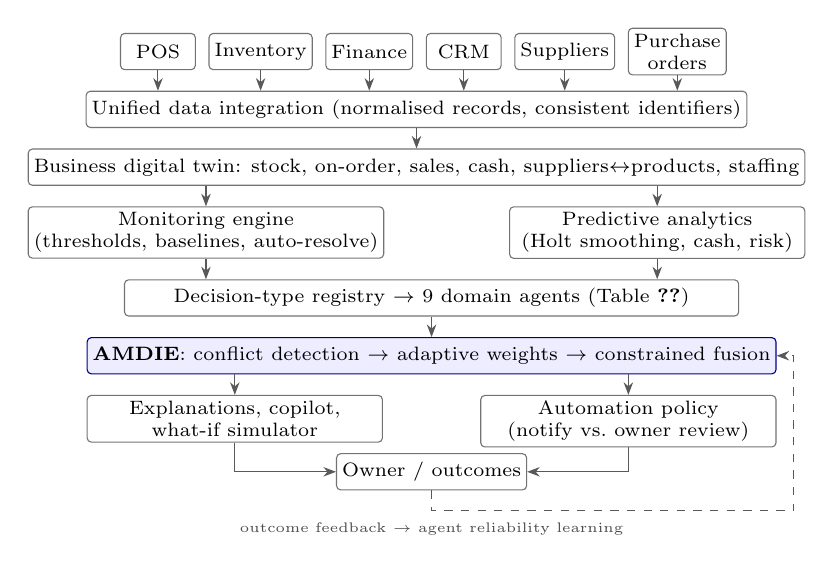
\begin{tikzpicture}[
  font=\scriptsize, node distance=2.6mm,
  box/.style={draw=black!55, rounded corners=1.5pt, align=center, inner sep=2pt, minimum height=4.6mm},
  src/.style={box, minimum width=9.5mm},
  wide/.style={box, minimum width=78mm},
  half/.style={box, minimum width=37.5mm},
  arr/.style={-{Stealth[length=1.6mm]}, black!65},
  hl/.style={box, fill=blue!7, draw=blue!55!black}
]
\node[src] (pos) {POS};
\node[src, right=1.6mm of pos] (inv) {Inventory};
\node[src, right=1.6mm of inv] (fin) {Finance};
\node[src, right=1.6mm of fin] (crm) {CRM};
\node[src, right=1.6mm of crm] (sup) {Suppliers};
\node[src, right=1.6mm of sup] (po) {Purchase\\orders};
\node[wide, below=of $(crm.south)!0.5!(fin.south)$] (int) {Unified data integration (normalised records, consistent identifiers)};
\node[wide, below=of int] (twin) {Business digital twin: stock, on-order, sales, cash, suppliers$\leftrightarrow$products, staffing};
\node[half, below=of twin.south west, anchor=north west] (mon) {Monitoring engine\\(thresholds, baselines, auto-resolve)};
\node[half, below=of twin.south east, anchor=north east] (pred) {Predictive analytics\\(Holt smoothing, cash, risk)};
\node[wide, below=of $(mon.south)!0.5!(pred.south)$] (agents) {Decision-type registry $\rightarrow$ 9 domain agents (Table~\ref{tab:registry})};
\node[wide, hl, below=of agents] (amdie) {\textbf{AMDIE}: conflict detection $\rightarrow$ adaptive weights $\rightarrow$ constrained fusion};
\node[half, below=of amdie.south west, anchor=north west] (xai) {Explanations, copilot,\\what-if simulator};
\node[half, below=of amdie.south east, anchor=north east] (auto) {Automation policy\\(notify vs.\ owner review)};
\node[box, below=10mm of amdie, minimum width=24mm] (owner) {Owner / outcomes};
\foreach \s in {pos,inv,fin,crm,sup,po} \draw[arr] (\s.south) -- (\s.south |- int.north);
\draw[arr] (int) -- (twin);
\draw[arr] (twin.south -| mon.north) -- (mon);
\draw[arr] (twin.south -| pred.north) -- (pred);
\draw[arr] (mon.south) -- (mon.south |- agents.north);
\draw[arr] (pred.south) -- (pred.south |- agents.north);
\draw[arr] (agents) -- (amdie);
\draw[arr] (amdie.south -| xai.north) -- (xai);
\draw[arr] (amdie.south -| auto.north) -- (auto);
\draw[arr] (xai.south) |- (owner.west);
\draw[arr] (auto.south) |- (owner.east);
\draw[arr, dashed] (owner.south) -- ++(0,-2.6mm) coordinate (fb) -- (fb -| {$(amdie.east)+(2.2mm,0)$}) |- (amdie.east);
\node[font=\tiny, text=black!70, below=0.3mm of fb, anchor=north] {outcome feedback $\rightarrow$ agent reliability learning};
\end{tikzpicture}
\caption{BizTwin AI architecture as implemented. Stock events from the monitoring engine trigger \amdie{} automatically; realised outcomes update agent reliability.}
\label{fig:arch}
\end{figure}

\textbf{Twin, monitoring and forecasting.} The twin is a read-only snapshot over the operational database, including on-order stock from open purchase orders and supplier-to-product links. A scheduler scans all tenants every five minutes for stock depletion, cash shortfall, sales spikes relative to a 14-day baseline, and unreliable suppliers; events close automatically when the condition clears, and stock events trigger an \amdie{} reorder cycle. Demand is forecast with Holt's additive-trend exponential smoothing on the 90 preceding complete days~\cite{hyndman2021}.

\textbf{Decision types and agents.} Each decision type has a registered set of agents and a single numeric axis (Table~\ref{tab:registry}); agents that serve several types (Sales, Finance, Marketing) project their view onto the axis of the decision at hand, so fusion never mixes units. Signed axes (price, staffing) allow negative recommendations. A Risk agent acts as a modifier under a risk-averse goal rather than as a voter.

\begin{table}[t]
\centering\scriptsize
\caption{Decision registry: participating agents and decision axis}
\label{tab:registry}
\setlength{\tabcolsep}{3pt}
\begin{tabular}{@{}lll@{}}
\toprule
Decision type & Agents & Axis \\
\midrule
Reorder quantity & Inventory, Sales, Finance, Procurement & units $\geq 0$ \\
Price adjustment & Pricing, Sales (+ Risk modifier) & price $\Delta$ (signed) \\
Promotion & Marketing, Finance & discount $\in[0,1]$ \\
Staffing & HR, Sales, Finance & hours $\Delta$ (signed) \\
Customer retention & Customer mgmt., Sales, Marketing & level $\in[0,1]$ \\
\bottomrule
\end{tabular}
\end{table}

\textbf{Explanation and automation.} Each decision is logged with every agent's recommendation, rationale, weight components and solver trace; the explanation endpoint and the copilot answer from this log and from the twin. Autonomous decisions pass an automation policy: reorders below a cost limit are dispatched as notifications, while pricing, staffing and costly actions wait for owner approval. A what-if simulator re-applies the forecasting models to an in-memory copy of the state and reports its assumptions (e.g.\ an elasticity estimated from the product's own price history).

%======================================================================
\section{AMDIE: Adaptive Multi-Agent Decision Fusion}
For a decision of type $k$ on product $p$, each registered agent $i$ returns a recommendation $r_i$ on the axis of $k$, a confidence $c_i\in[0,1]$, a risk score $\rho_i\in[0,1]$, a rationale, and optionally a hard cap $\bar u_i$ (e.g.\ Finance's affordable quantity).

\textbf{Conflict detection.} The conflict score is
\begin{equation}
\kappa=\min\Bigl(1,\max_{i<j}\frac{|r_i-r_j|}{\max(|r_i|,|r_j|,1)}\Bigr),
\end{equation}
and a conflict is flagged when $\kappa>\tau_c=0.3$; it is reported to the owner and recorded for audit.

\textbf{Adaptive weights.} Each agent receives the score
\begin{equation}
s_i = w_1R_i + w_2c_i + w_3H_i + w_4C_i - w_5\rho_i - w_6D_i,
\end{equation}
where $R_i$ is an exponentially smoothed reliability, $H_i$ the mean historical accuracy, $C_i$ the cosine similarity between a sentence embedding~\cite{reimers2019} of the decision context and the agent's domain description, and $D_i=\min(1,|r_i-\tilde r|/\max(|\tilde r|,1))$ the deviation from the median recommendation $\tilde r$. Weights are
\begin{equation}
\pi_i=\frac{\exp(s_i/T)}{\sum_j\exp(s_j/T)}.
\end{equation}
Because $s_i$ lies in a narrow range, $T=1$ yields nearly uniform weights; a small $T$ makes the scheme an exponential-weights rule over reliability~\cite{freund1997}.

\textbf{Service-level-aware outcome learning.} When a decision's outcome $y$ is known (for replenishment, the ex-post order quantity that would have exactly covered demand), each agent's accuracy is scored with the pinball loss at level $q$:
\begin{equation}
a_i=1-\frac{q\,(y-r_i)^+ + (1-q)\,(r_i-y)^+}{\max(q,1-q)\,\max(|r_i|,|y|,1)} .
\end{equation}
For $q=0.5$ this is the symmetric relative error; for $q>0.5$ under-ordering (lost sales) is penalised more than over-ordering, which is the newsvendor optimality condition~\cite{koenker1978,zipkin2000}. $q$ is an owner-level service target. Reliability is updated as $R_i\leftarrow 0.3\,a_i+0.7\,R_i$, and after 30 outcomes the coefficients $w_{1..6}$ are refitted by non-negative least squares of $a_i$ on the score components, per tenant and decision type.

\textbf{Constrained fusion.} The fused decision solves the LP (HiGHS~\cite{huangfu2018})
\begin{align}
\max_{x,\,u}\;& \textstyle\sum_i \pi_i u_i \;-\; \lambda_c x \;+\; \lambda_t\min(x,\hat d) \label{eq:lp}\\
\text{s.t.}\;& u_i\le 1-|x-r_i|/\sigma_i,\quad 0\le u_i\le1, \notag\\
& \ell_k\le x\le \min(U_k,\min_i\bar u_i),\quad \text{unit cost}\cdot x\le B, \notag
\end{align}
with triangular utilities of half-width $\sigma_i=(0.4|r_i|+\delta)/c_i$, axis bounds $[\ell_k,U_k]$, budget $B$, and goal-dependent cost and turnover terms $\lambda_c,\lambda_t$ (zero under profit maximisation).

\begin{proposition}
If $\lambda_c=\lambda_t=0$ and the optimum lies within every agent's utility support, the solution of \eqref{eq:lp} is a weighted median of $\{r_i\}$ with weights $\pi_i/\sigma_i$, clipped to the feasible interval.
\end{proposition}
\begin{IEEEproof}[Sketch]
At the optimum $u_i=1-|x-r_i|/\sigma_i$, so the objective is $\sum_i\pi_i-\sum_i(\pi_i/\sigma_i)|x-r_i|$, a convex piecewise-linear function of $x$ minimised at the weighted median; feasibility constraints clip it.
\end{IEEEproof}
The fused value therefore never lies outside the range of agent recommendations, and, because $\sigma_i$ grows with $|r_i|$, agents recommending larger values receive proportionally less influence. Algorithm~\ref{alg:amdie} summarises one cycle.

\begin{algorithm}[t]
\caption{One \amdie{} cycle for decision type $k$}
\label{alg:amdie}
\footnotesize
\begin{algorithmic}[1]
\State $\mathcal{A}\gets$ agents registered for $k$; query each for $(r_i,c_i,\rho_i,\bar u_i)$ on axis $k$
\State compute $\kappa$; flag conflict if $\kappa>\tau_c$
\State compute $s_i$ from stored $R_i,H_i$ and $C_i,\rho_i,D_i$; $\pi\gets\mathrm{softmax}(s/T)$
\State adjust $\pi$ for the owner's goal; solve LP \eqref{eq:lp} for $x^\star$
\State log trace, generate explanation, route $x^\star$ through automation policy
\State \textbf{on outcome} $y$: update $a_i, R_i, H_i$; refit $w$ if $\geq 30$ outcomes
\end{algorithmic}
\end{algorithm}

%======================================================================
\section{Experimental Setup}
Only replenishment has an objective, simulable ground truth, so we evaluate \amdie{} on reorder quantity. Pricing, promotion, staffing and retention decisions are executed by the same pipeline but would require field data or controlled experiments to evaluate.

\textbf{Environment.} A seeded retailer with 8 products, 120 days of history and a 140-day test horizon reviewed weekly (20 cycles). Daily demand is $d_t\sim\mathcal N(\mu_t,(v\mu_t)^2)$, rounded and floored at zero, with $\mu_t=b(1+g\,t/365)(1+0.25\sin\frac{2\pi t}{7})(1+a\sin(\frac{2\pi t}{365}+\phi))$ and product-specific $b,g,a,\phi,v$. Lead times are stochastic per order. Unmet demand is lost; holding cost is 25\% of unit cost per year; each order line costs 15; orders are paid on placement and truncated to a shared weekly purchase budget and available cash. Only censored sales are recorded, as a POS would. Three scenarios vary the conditions: \emph{baseline} (budget 1.5$\times$ expected cost of goods, $v\in[0.2,0.4]$), \emph{tight budget} (0.8$\times$), and \emph{volatile} ($v\in[0.4,0.7]$, a 3-week demand surge or drop for half the products, doubled lead-time variance, 30\% unreliable suppliers).

\textbf{Same code path.} Agent policies call the production agents and \amdie{} calls the API's decision function against the simulator's database; orders are written as purchase orders, so agents see on-order stock. After each order's protection interval, the ex-post quantity is fed back as the outcome, as the outcome endpoint does in deployment.

\textbf{Policies.} \emph{Newsvendor} and \emph{base-stock} (95\% cycle service) order-up-to policies on observed sales~\cite{zipkin2000}; each \emph{single agent}; the unweighted \emph{mean} and \emph{median} of the four agents; \amdie{}; seven ablations; and a perfect-foresight order-up-to reference that knows future demand and lead times (not an upper bound, since it holds no buffer for the next order's lead time).

\textbf{Protocol.} Policies run on identical instances (common random numbers), so comparisons are paired. The softmax temperature $T\in\{1,0.2,0.05,0.02\}$ and service level $q\in\{0.5,0.9\}$ were selected on four development seeds per scenario ($T=0.05$, $q=0.9$); all reported results use 10 different held-out seeds per scenario (510 runs). The primary metric is profit (revenue minus purchases, holding and ordering cost, plus the change in inventory value) relative to base-stock on the same instance. We report means with 95\% CIs and paired $t$-tests across seeds with Holm correction within each scenario; product-level Wilcoxon tests agree in direction. An \amdie{} decision takes 0.26\,s on a desktop CPU.

%======================================================================
\section{Results}
\begin{figure*}[t]
\centering
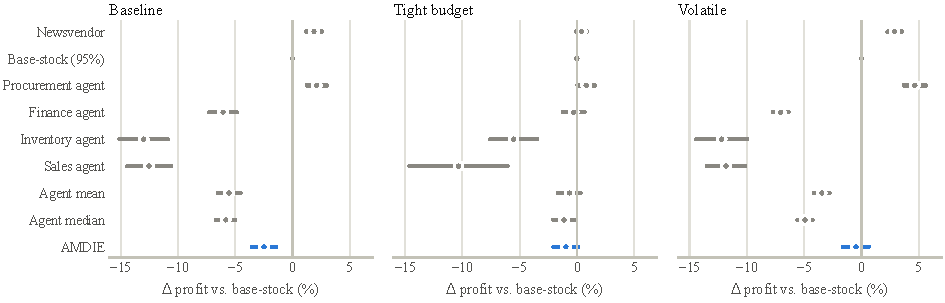
\includegraphics[width=\textwidth]{figures/profit.pdf}
\caption{Profit relative to the base-stock policy on the same instance (mean and 95\% CI over 10 held-out instances per scenario).}
\label{fig:profit}
\end{figure*}

\begin{table*}[t]
\centering\footnotesize
\caption{Profit relative to base-stock (\%, mean [95\% CI]) and fill rate, 10 held-out instances per scenario}
\label{tab:main}
\begin{tabular}{@{}lcccccc@{}}
\toprule
& \multicolumn{2}{c}{Baseline} & \multicolumn{2}{c}{Tight budget} & \multicolumn{2}{c}{Volatile} \\
\cmidrule(lr){2-3}\cmidrule(lr){4-5}\cmidrule(l){6-7}
Method & $\Delta$ profit & Fill & $\Delta$ profit & Fill & $\Delta$ profit & Fill \\
\midrule
Newsvendor order-up-to          & $+1.88$ [$+1.20$, $+2.57$]   & 0.970 & $+0.42$ [$-0.04$, $+0.87$]  & 0.735 & $+2.90$ [$+2.29$, $+3.51$]   & 0.928 \\
Base-stock (95\% service)       & 0                            & 0.951 & 0                           & 0.733 & 0                            & 0.900 \\
Procurement agent only          & $+2.12$ [$+1.25$, $+3.00$]   & 0.972 & $+0.81$ [$+0.06$, $+1.56$]  & 0.737 & $+4.67$ [$+3.69$, $+5.64$]   & 0.947 \\
Finance agent only              & $-6.06$ [$-7.25$, $-4.86$]   & 0.894 & $-0.29$ [$-1.23$, $+0.66$]  & 0.729 & $-7.04$ [$-7.73$, $-6.36$]   & 0.836 \\
Inventory agent only            & $-12.99$ [$-15.09$, $-10.89$]& 0.827 & $-5.53$ [$-7.57$, $-3.50$]  & 0.699 & $-12.20$ [$-14.42$, $-9.99$] & 0.792 \\
Sales agent only                & $-12.52$ [$-14.42$, $-10.61$]& 0.824 & $-10.34$ [$-14.62$, $-6.05$]& 0.664 & $-11.82$ [$-13.49$, $-10.15$]& 0.791 \\
Agent mean                      & $-5.53$ [$-6.52$, $-4.54$]   & 0.900 & $-0.65$ [$-1.63$, $+0.32$]  & 0.728 & $-3.47$ [$-4.16$, $-2.77$]   & 0.871 \\
Agent median                    & $-5.83$ [$-6.65$, $-5.00$]   & 0.896 & $-1.13$ [$-2.07$, $-0.19$]  & 0.725 & $-4.93$ [$-5.58$, $-4.28$]   & 0.857 \\
\textbf{AMDIE}                  & $\mathbf{-2.48}$ [$-3.53$, $-1.42$] & 0.927 & $\mathbf{-0.96}$ [$-2.04$, $+0.12$] & 0.726 & $\mathbf{-0.47}$ [$-1.59$, $+0.65$] & 0.899 \\
\midrule
Perfect-foresight reference     & $-3.07$ [$-4.67$, $-1.47$]   & 0.924 & $+0.05$ [$-1.04$, $+1.14$]  & 0.731 & $-5.90$ [$-8.06$, $-3.75$]   & 0.848 \\
\bottomrule
\end{tabular}
\end{table*}

Table~\ref{tab:main} and Fig.~\ref{fig:profit} summarise the comparison.

\textbf{Against naive multi-agent aggregation.} \amdie{} outperforms the unweighted agent mean by $+3.05$\,pp (baseline, 9/10 instances, $p_{\text{Holm}}=0.006$) and $+2.99$\,pp (volatile, 10/10, $p_{\text{Holm}}=0.014$), and the agent median by $+3.35$ and $+4.45$\,pp ($p_{\text{Holm}}\le0.002$). It also outperforms the Finance, Inventory and Sales agents in both scenarios ($p_{\text{Holm}}<0.01$).

\textbf{Against strong baselines.} \amdie{} does not reach the best single agent or the newsvendor policy. In the baseline scenario it trails base-stock by $2.48$\,pp, newsvendor by $4.36$\,pp and the Procurement agent by $4.60$\,pp (all $p_{\text{Holm}}<0.01$). In the volatile scenario it is statistically indistinguishable from base-stock ($-0.47$\,pp, $p_{\text{Holm}}=0.73$) but trails newsvendor and Procurement. Under the tight budget, truncation by the budget dominates every policy (fill rates 0.66--0.74, 30--38\% of orders truncated), and no AMDIE comparison except against Procurement ($-1.77$\,pp) and the two weakest agents is significant after correction.

\textbf{Learned trust.} Fig.~\ref{fig:weights} shows that \amdie{} starts by trusting the Sales agent (high self-reported confidence) and, as outcomes arrive, shifts 70--80\% of its weight to Procurement---the agent with the best realised profit---within four review cycles; the same pattern holds in all three scenarios. Agents disagreed on 99\% of decisions ($\kappa>0.3$), so the conflict flag is not informative at the current threshold.

\begin{figure}[t]
\centering
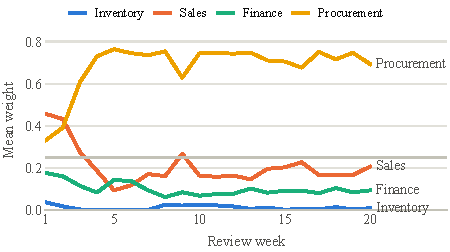
\includegraphics[width=\columnwidth]{figures/weights.pdf}
\caption{Mean \amdie{} weight per agent over the review cycles (baseline scenario, 10 instances). Grey line: uniform weight.}
\label{fig:weights}
\end{figure}

\textbf{Ablation.} Table~\ref{tab:ablation} removes one component at a time. Adaptive weighting and outcome learning are essential: equal weights cost 2.9 and 5.1\,pp, freezing reliability 1.6 and 2.5\,pp, and the untuned configuration ($T=1$, $q=0.5$) is as poor as equal weights, confirming that a flat softmax neutralises the weighting. Two components hurt: replacing the LP by a weighted average gains $+2.2$ and $+2.4$\,pp, and removing the divergence penalty gains $+1.9$ and $+1.4$\,pp. Context relevance and Finance's hard cap have no measurable effect in this setting, because the shared budget, not the per-product cap, is binding.

\begin{table}[t]
\centering\footnotesize
\caption{Ablation: change in profit (pp of base-stock profit) when a component is removed; $^\ast$ $p_{\text{Holm}}<0.05$}
\label{tab:ablation}
\setlength{\tabcolsep}{4pt}
\begin{tabular}{@{}lccc@{}}
\toprule
Removed component & Baseline & Tight & Volatile \\
\midrule
Tuning ($T{=}1$, $q{=}0.5$)          & $-2.78^\ast$ & $+0.55$ & $-4.85^\ast$ \\
Adaptive weights (equal)             & $-2.92^\ast$ & $+0.77$ & $-5.10^\ast$ \\
Outcome learning                     & $-1.64^\ast$ & $+0.50$ & $-2.52^\ast$ \\
LP fusion (weighted average)         & $+2.23^\ast$ & $+0.75$ & $+2.38^\ast$ \\
Divergence penalty                   & $+1.89^\ast$ & $+0.97$ & $+1.40^\ast$ \\
Context relevance                    & $-0.34$      & $+0.37$ & $-0.58$ \\
Finance hard cap                     & $0.00$       & $0.00$  & $0.00$ \\
\bottomrule
\end{tabular}
\end{table}

%======================================================================
\section{Discussion and Limitations}
\textbf{Why AMDIE helps.} The four agents differ by up to 15\,pp in profit, and which one is best is not known in advance. Exponential weighting over a service-aware reliability signal identifies the strongest agent from operational outcomes alone, which is why \amdie{} recovers most of the gap between the naive ensembles and the best agent, consistent with the online-learning view of expert combination~\cite{freund1997}.

\textbf{Why it falls short.} The remaining gap has an identifiable cause. By Proposition~1, the LP returns a weighted median with weights $\pi_i/\sigma_i$, and $\sigma_i$ grows with $|r_i|$; the divergence penalty likewise down-weights agents far from the median. The best agent in this domain is the one that holds the most safety stock, so both mechanisms pull the decision toward the more conservative agents: \amdie{}'s fill rate (0.927) lies between the ensemble (0.900) and Procurement (0.972). Removing either mechanism improves profit, which points to a weighted-average fusion without the outlier penalty as the next version. Because this was observed on the test instances, it must be confirmed on fresh instances before being claimed. The newsvendor policy is the right model for this simulated environment by construction; \amdie{}'s value lies in combining heterogeneous agents across decision types with an auditable trace, not in beating a correctly specified single-item policy. Our results also echo the forecast-combination literature: estimated weights help only when agents differ substantially~\cite{smith2009}, as the tight-budget scenario illustrates.

\textbf{Limitations.} The evaluation is simulated, covers one decision type, and uses synthetic demand, so field validation with SME data remains necessary. An LLM decision-maker baseline is implemented but was not completed within free-tier API limits. No user study of the explanations or copilot has been conducted. The conflict threshold needs calibration per decision type. The twin consolidates sensitive financial and customer data; the implementation uses role-based access and encrypted cost fields, but a full governance assessment is outside our scope.

%======================================================================
\section{Conclusion}
BizTwin AI implements a business control tower in which nine domain agents are coordinated by \amdie{}. In 510 paired simulation runs, adaptive, outcome-trained weighting clearly beats unweighted agent aggregation and matches a base-stock policy under volatile conditions, while two fusion components introduce a conservative bias that keeps it below the best single agent and the newsvendor policy. Future work will (i) validate weighted-average fusion without the outlier penalty on fresh instances, (ii) complete the LLM-agent baseline, (iii) evaluate pricing and staffing decisions with field data, and (iv) study explanation quality with SME owners. This work supports UN Sustainable Development Goal 8 (decent work and economic growth).

\bibliographystyle{IEEEtran}
\bibliography{refs}

\end{document}
